% !TeX root = ../translation.tex

\newpage

\section{引言}

生成对抗网络(GAN)已成为无条件图像生成的主要方法之一。当在多个数据集上进行训练时,GAN能够产生逼真的和视觉上吸引人的样本。GAN方法训练了一个从随机噪声中回归真实图像的无条件的生成器,以及一个测量生成的样本和真实图像之间的差异的鉴别器。GAN已经经过多次改进。其中一个突破是将最优传输(OT)理论与GAN相结合,如Wasserstein GAN(WGAN)[1]。在WGAN框架中,生成器计算了从白噪声到数据分布的OT映射,而判别器计算了真实数据分布与生成数据分布之间的Wasserstein距离。

\subsection{流形分布假设}

GAN的成功可以通过以下事实进行解释,即GAN
有效地发现了真实数据集的内在结构。该结构可以用流形分布假设来表示,即一类特定的自然数据主要集中在一个低维流形上,且该低维流形被嵌入高维背景空间[2]。

图 \ref{fig:1} 显示了MNIST数据库的流形结构。每个手写数字图像具有尺寸$28 \times 28$,并被视为$\mathbb{R}^{784}$图像空间中的一个点。MNIST数据库集中在一个低维(2维流形)附近。通过使用t-SNE流形嵌入算法[3],MNIST数据集被映射到一个平面域上,每个图像被映射到一个点上。代表相同数字的图像被映射到同一个簇上,10个簇分别被不同的颜色编码。这表明MNIST数据集分布在一个二维(2D)曲面附近,该曲面被嵌入在$\mathbb{R}^{784}$的单位超立方体中。

\begin{figure}[h]
	\centering
	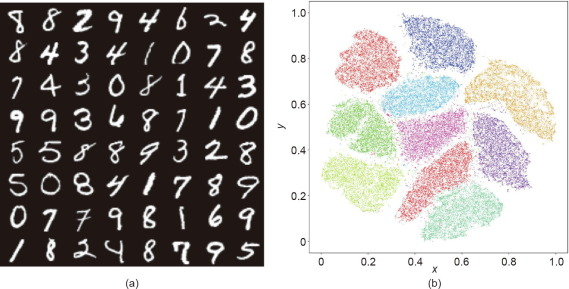
\includegraphics[width=0.6\linewidth]{1.jpg}
	
	\caption{MNIST数据集的流形分布。(a)MNIST数据集中的手写数字;(b)利用t-SNE算法得到的2D平面内数字的嵌入结果。将x和y相对坐标进行标准化。}
	\label{fig:1}
\end{figure}

\subsection{GAN理论模型}

图 \ref{fig:2} 为GAN的理论模型。真实的数据分布$\nu$主要集中在被嵌入背景空间$chi$中的流形$\sum$上。$(\sum,\nu)$
一起显示了真实数据集的内在结构。GAN模型计算一个从隐空间$Z$到流形$\sum$的解码映射$g_{\theta}$,其中,$\theta$表示深度神经网络(DNN)参数。$\zeta$是隐空间中的Gaussian分布,$g_{\theta}$将$\zeta$前推为$\nu_{\theta}$。判别器计算了真实数据分布$\nu$和生成数据分布$\mu_{\theta}$之间的距离,如Wasserstein距离$W_c(\mu_{\theta},\nu)$,其等价于Kontarovich势能$\varphi_{\xi}$。

\begin{figure}[h]
	\centering
	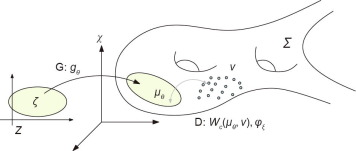
\includegraphics[width=0.6\linewidth]{2.jpg}
	\caption{GAN的理论模型。G:生成器;D:判别器。}
	\label{fig:2}
\end{figure}

尽管GAN有许多优点,但它们也有严重的缺点。在理论上,我们对深度学习的基本原则的理解仍然是原始的。在实践中,GAN的训练是棘手的,其对超参数是敏感的;而且GAN经常会遇到模式崩溃问题。最近,Meschede等人[4]研究了9种不同的GAN模型及其变体,结果表明,基于梯度下降的GAN优化并不总是局部收敛的。

根据流形分布假设,自然数据集可以被表示为关于
流形的概率分布。因此,GAN主要完成两项任务:\ding{172}流形学习,即计算隐空间与背景空间之间的解码映射和编码映射;\ding{173}概率变换,即在隐空间或图像空间中计算白噪声与数据分布之间的变换。

图 \ref{fig:3} 为生成器映射$g_{theta}=ℎ \circ T$的分解,其中$h: Z \to \sum$ 为从隐空间到背景空间中的数据流形$\sum$的解码映射,$T: Z\to Z$是概率分布变换映射。流形学习的解码映射是$h$,测度变换映射是$T$。

\begin{figure}[h]
	\centering
	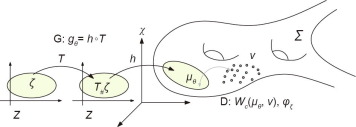
\includegraphics[width=0.6\linewidth]{3.jpg}
	\caption{生成器映射被分解为解码映射$h$和概率分布变换映射$T$。$T_{\#}\chi$是由$T$推导出的前推测度。
	}
	\label{fig:3}
\end{figure}

\subsection{OT观点}

OT理论[5]研究了以最经济的方式将一种概率分布转化为另一种概率分布的问题。OT提供了严格而强大的方法来计算最优映射,这些方法将一个概率分布转换为另一个分布,同时计算出它们之间的距离[6]。

如前所述,GAN完成了两个主要任务:流形学习和概率分布变换。后一项任务可以直接通过OT方法完成。具体地说,在图3中,可以用OT理论计算出概率分布变换映射$T$。判别器计算了生成数据分布与真实数据分布之间的Wasserstein距离$W_c(\mu_{\theta},\nu)$,可以用OT方法直接计算。

从理论的角度来看,GAN可以由OT理论来解释,从
而使得一部分黑匣子变得透明,同时将概率分布变换过程简化为一个凸优化过程。OT理论使解的存在性和唯一性具有理论保证, 而且其收敛速度和近似程度也可以得到全面分析。

OT理论也解释了模式崩溃的根本原因。根据Monge-Ampère方程的正则性理论,变换映射在某些奇异集上是不连续的。然而,DNN只能表达连续函数和连续映射。因此,目标变换映射位于GAN所表示的函数空间之外。这种内在的冲突使得模式崩溃问题不可避免。

OT解释还揭示了更复杂的生成器和判别器之间的
关系。在现有的GAN模型中,生成器和判别器之间是相互竞争的,它们不共享中间的计算结果。OT理论表明,在$L^2$成本函数下,生成器和判别器的最优解可以用
闭合式来相互表示。因此,生成器与判别器之间的关系应该是相互协作的而不是相互竞争的,而且它们应该共享中间的计算结果以提高计算效率。

\subsection{自动编码器-最优传输模型}

为了降低GAN的训练难度,特别是为了避免模式崩溃,我们提出了一个基于OT理论的更简单的生成模型:一个自动编码器(AE)OT模型(AE-OT),如图 \ref{fig:4} 所示。

\begin{figure}[h]
	\centering
	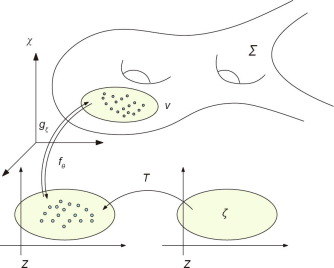
\includegraphics[width=0.6\linewidth]{4.jpg}
	\caption{生成模型AE-OT,将AE和OT相结合。
	}
	\label{fig:4}
\end{figure}

如前所述,生成模型的两个主要任务是流形学习和概率分布变换。AE计算了编码映射$f_{\theta}:Z \to \sum$,和解码映射$g_{\xi}: \sum \to Z$,目的是用于流形学习。OT映射$T:Z \to Z$,将白噪声$\zeta$转换为由编码映射$(f_{\theta})_{\#}\nu$前推的数据分布。

AE-OT模型有很多优点。从理论的角度来看,OT理论已经建立和得到了人们充分的理解。通过对解码映射和OT映射进行解耦,可以提高生成模型的理论严谨性,使一部分黑盒透明。在实际应用中,将OT映射简化为一个凸优化问题,保证了解的存在性和唯一性,同时使训练过程不会陷入局部最优状态。与OT映射相关的凸能量具有显式的Hessian矩阵结构;因此,我们可以采用二阶收敛的牛顿方法,或采用超线性收敛的拟牛顿方法进行优化。相比之下,目前的生成模型基于线性收敛的梯度下降法。而且在AE-OT模型中,未知数个数与训练样本个数相同,从而避免了过参数化问题。在Monte Carlo方法中,采样密度可以完全控制OT映射的误差范围。具有自适应的层次算法进一步提高了效率。并行OT映射算法可以使用图形处理单元(GPU)实现。更重要的是,AE-OT模型可以消除模式崩溃问题。

\subsection{贡献}

本工作利用OT理论解释了GAN模型。GAN可以完成两个主要任务:流形学习和概率分布变换。后一种任务可以使用OT方法来完成。生成器计算了OT映射,而判别器计算生成的数据分布和真实数据分布之间的Wasserstein距离。利用Brenier定理,我们可以将生成器和判别器之间的竞争关系用协作关系来代替;根据Monge-Ampère方程的正则性理论,分布变换映射的不连续性导致了模式崩溃。我们进一步提出,利用AE-OT模型来解耦流形学习和概率分布变换,从而使部分黑匣子透明化、提高训练效率以及避免模式崩溃。实验结果表明了我们所提出的方法的有效性。

本文的组织结构如下:第2节简要回顾了OT和GAN中相关的工作;第3节简要介绍了OT的基本理论和Monge-Ampère方程的正则性理论;第4节介绍了一种适合深度学习设置的用于计算OT的变分框架;第5节从OT的角度分析了GAN模型,解释了生成器与判别器之间的协作关系(不是竞争关系),以及揭示了模式崩溃的内在原因;第6部分总结了实验结果;第7部分对全文进行了总结。。